% ------------------------------------------------------------------------------
% TYPO3 CMS 6.2 LTS - What's New - Chapter "Backend Changes" (Russian Version)
%
% @author	Andrey Aksenov <aksenovaa@bk.ru>
% @license	Creative Commons BY-NC-SA 3.0
% @link		http://typo3.org/download/release-notes/whats-new/
% @language	Russian
% ------------------------------------------------------------------------------
% Chapter: Backend Changes
% ------------------------------------------------------------------------------

\section{Изменение во внутреннем интерфейсе}
\begin{frame}[fragile]
	\frametitle{Изменение во внутреннем интерфейсе}

	\begin{center}\huge{Глава 3:}\end{center}
	\begin{center}\huge{\color{typo3darkgrey}\textbf{Изменение во внутреннем интерфейсе}}\end{center}

\end{frame}

% ------------------------------------------------------------------------------
% Autofocus
% ------------------------------------------------------------------------------
% http://forge.typo3.org/issues/49228

\begin{frame}[fragile]
	\frametitle{Изменение во внутреннем интерфейсе}
	\framesubtitle{Авторизация}

 	\begin{itemize}
		\item Автоматически в фокусе оказывается поле "имя пользователя" (username)\newline
			(HTML5 атрибут: \texttt{autofocus="autofocus"})
	\end{itemize}

	\begin{figure}
		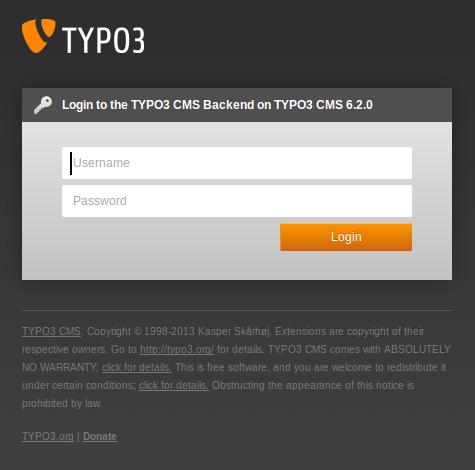
\includegraphics[width=0.4\linewidth]{Images/BackendChanges/BackendLogin.png}
	\end{figure}

\end{frame}

% ------------------------------------------------------------------------------
% Visual Appearance
% ------------------------------------------------------------------------------
% http://forge.typo3.org/issues/48376

\begin{frame}[fragile]
	\frametitle{Изменение во внутреннем интерфейсе}
	\framesubtitle{Внешний вид}

	\begin{columns}[T]

		\begin{column}{.5\textwidth}
			\begin{itemize}
				\item Макет стал удобнее и оживился
				\item Уменьшены отступы между элементами модуля (левый столбец)
				\item В основе лежит 12-колонная сетка, удвоенная
			\end{itemize}

			\advance\leftskip+3.8cm

            \smaller
                Слева: TYPO3 4.5\newline
                Справа: TYPO3 6.2
            \normalsize
		\end{column}

		\begin{column}{.5\textwidth}
			\begin{figure}\vspace*{-0.4cm}
				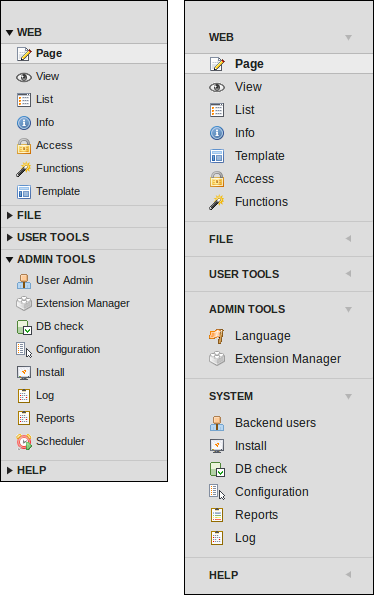
\includegraphics[width=0.6\linewidth]{Images/BackendChanges/VisualAppearance.png}
			\end{figure}
		\end{column}

	\end{columns}

\end{frame}

% ------------------------------------------------------------------------------
% Visual Appearance
% ------------------------------------------------------------------------------

\begin{frame}[fragile]
	\frametitle{Изменение во внутреннем интерфейсе}
	\framesubtitle{Внешний вид}

	\begin{columns}[T]

		\begin{column}{.5\textwidth}

			\begin{itemize}
				\item Изменена структура модулей в левом столбце
				\item Разделен на две части модуль "Инструменты управления" ("Admintools"):

					\begin{itemize}
						\item \textbf{Инструменты управления – Admintools} ("Языки"/"Languages" и "Расширения"/"Extension
						Manager")
						\item \textbf{Система – System} (низкоуровневые инструменты, без столбца дерева страниц)
					\end{itemize}

				\item Удален модуль "Справка TypoScript"/"TypoScript Help" (устарел)
				"TypoScript-Help"

			\end{itemize}

		\end{column}

		\begin{column}{.5\textwidth}
			\begin{figure}\vspace*{-0.4cm}
				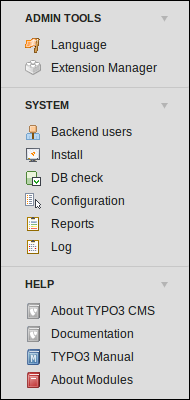
\includegraphics[width=0.35\linewidth]{Images/BackendChanges/AdminTools.png}
			\end{figure}
		\end{column}

	\end{columns}

\end{frame}

% ------------------------------------------------------------------------------
% Visual Appearance
% ------------------------------------------------------------------------------
% http://forge.typo3.org/issues/36017

\begin{frame}[fragile]
	\frametitle{Изменение во внутреннем интерфейсе}
	\framesubtitle{Внешний вид}

	\begin{itemize}
		\item \texttt{<h1>}-заголовки в основной области используют шрифт TYPO3 "Share"
	\end{itemize}

	\begin{figure}
		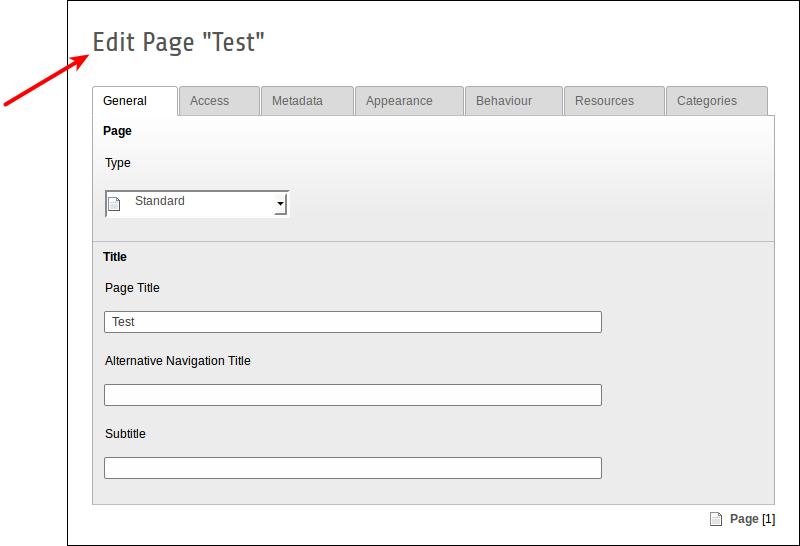
\includegraphics[width=0.6\linewidth]{Images/BackendChanges/ConsistantFont.png}
	\end{figure}

\end{frame}

% ------------------------------------------------------------------------------
% Visual Appearance
% ------------------------------------------------------------------------------
% http://forge.typo3.org/issues/41631

\begin{frame}[fragile]
	\frametitle{Изменение во внутреннем интерфейсе}
	\framesubtitle{Внешний вид}

	\begin{itemize}
		\item Новый значок для модуля "Отчёты"/"Reports"
	\end{itemize}

	\begin{figure}
		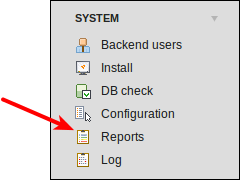
\includegraphics[width=0.35\linewidth]{Images/BackendChanges/ModuleReportsIcon.png}
	\end{figure}

\end{frame}

% ------------------------------------------------------------------------------
% Filelist: Drag&Drop File Upload
% ------------------------------------------------------------------------------
% http://forge.typo3.org/issues/47005

\begin{frame}[fragile]
	\frametitle{Изменение во внутреннем интерфейсе}
	\framesubtitle{Загрузка файлов перетаскиванием (1)}

	\begin{itemize}
		\item В списке файлов применен функционал HTML5 загрузки файлов перетаскиванием

	\end{itemize}

	\begin{figure}
		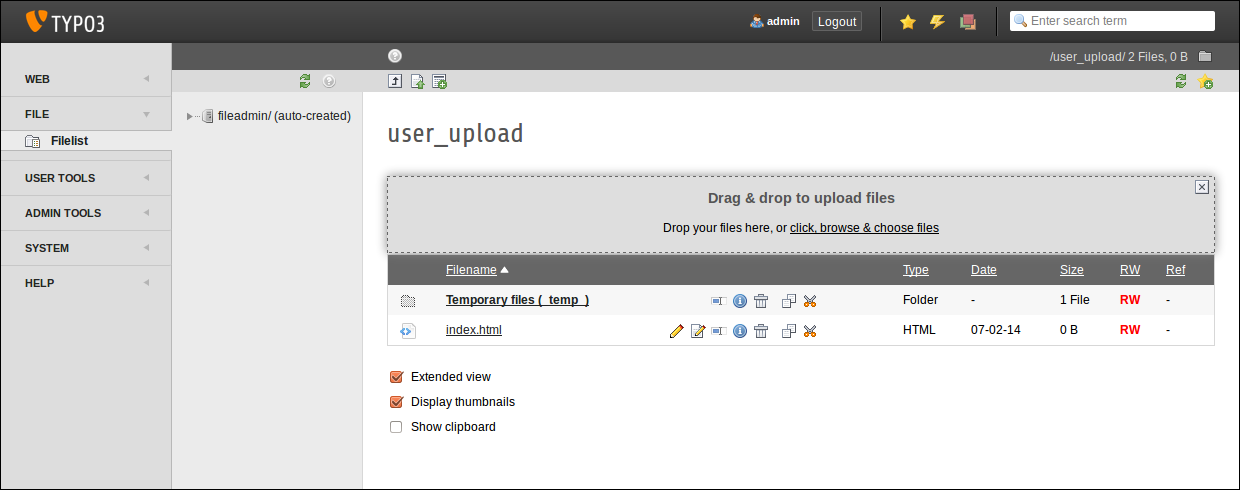
\includegraphics[width=0.95\linewidth]{Images/BackendChanges/DragDropFileUpload.png}
	\end{figure}

\end{frame}

% ------------------------------------------------------------------------------
% Drag&Drop File Upload Via Content Elements
% (slide added in March 2014)
% ------------------------------------------------------------------------------

\begin{frame}[fragile]
	\frametitle{Изменение во внутреннем интерфейсе}
	\framesubtitle{Загрузка файлов перетаскиванием (2)}

	\begin{itemize}
		\item ...и через элементы содержимого (кнопка: "Select \& upload files")

	\end{itemize}

	\begin{figure}
		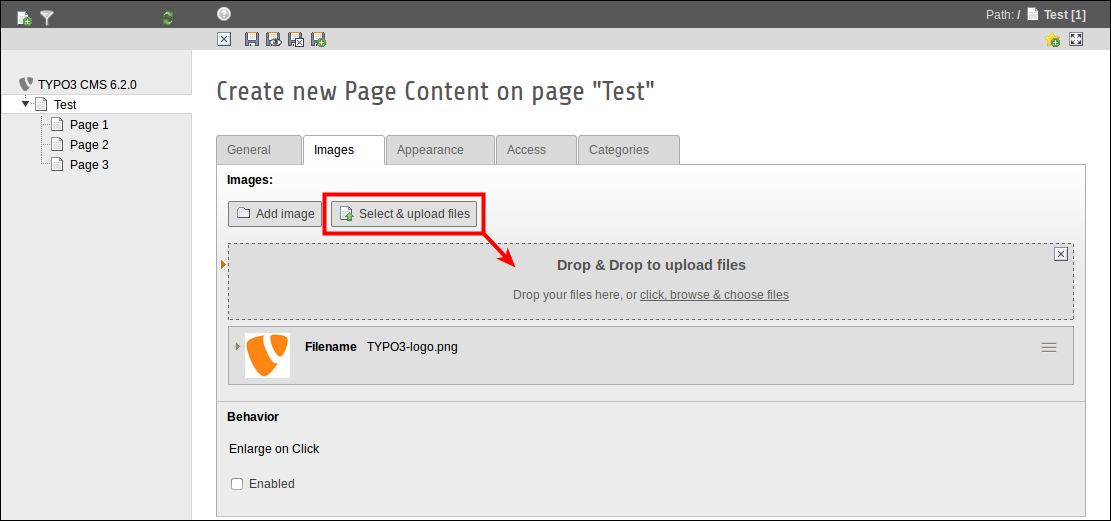
\includegraphics[width=0.95\linewidth]{Images/BackendChanges/SelectAndUploadFiles.png}
	\end{figure}

\end{frame}

% ------------------------------------------------------------------------------
% Backend Users
% ------------------------------------------------------------------------------
% http://forge.typo3.org/issues/43053

\begin{frame}[fragile]
	\frametitle{Изменение во внутреннем интерфейсе}
	\framesubtitle{Удобство: внутренние пользователи}

	\begin{itemize}
		\item Выводится имя пользователя и настоящее имя (первый столбец в режиме списка)
		\item Щёлкните по имени (пользователя) для его редактирования
		\item Удалена кнопка добавления в режиме списка

	\end{itemize}

	\begin{figure}
		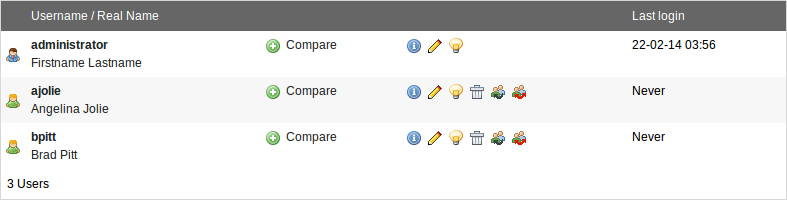
\includegraphics[width=0.95\linewidth]{Images/BackendChanges/BackendUserList.png}
	\end{figure}

\end{frame}

% ------------------------------------------------------------------------------
% Live Search
% ------------------------------------------------------------------------------
% http://forge.typo3.org/issues/35358

\begin{frame}[fragile]
	\frametitle{Изменение во внутреннем интерфейсе}
	\framesubtitle{Живой поиск}

	\begin{itemize}
		\item Подсказка в "живом поиске" показывает как UID, так и PID
		\item Если после поиска снова закрыть форму редактирования, то выводится режим списка для страницы (а не пустая страница)
	\end{itemize}

	\begin{figure}
		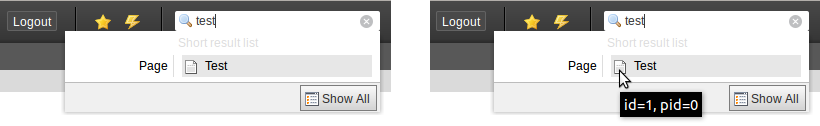
\includegraphics[width=0.8\linewidth]{Images/BackendChanges/LiveSearchTooltip.png}
	\end{figure}

\end{frame}

% ------------------------------------------------------------------------------
% Live Search
% ------------------------------------------------------------------------------

\begin{frame}[fragile]
	\frametitle{Изменение во внутреннем интерфейсе}
	\framesubtitle{Живой поиск}

	\begin{itemize}
		\item В TYPO3 < 6.2, для страниц учитывались лишь поля базы данных \texttt{title} и \texttt{uid}
		\item В TYPO3 >= 6.2, к поиску можно добавить поля \texttt{alias}\newline
			(требуется UserTSconfig: \texttt{options.pageTree.searchInAlias = 1})
	\end{itemize}

	\begin{figure}
		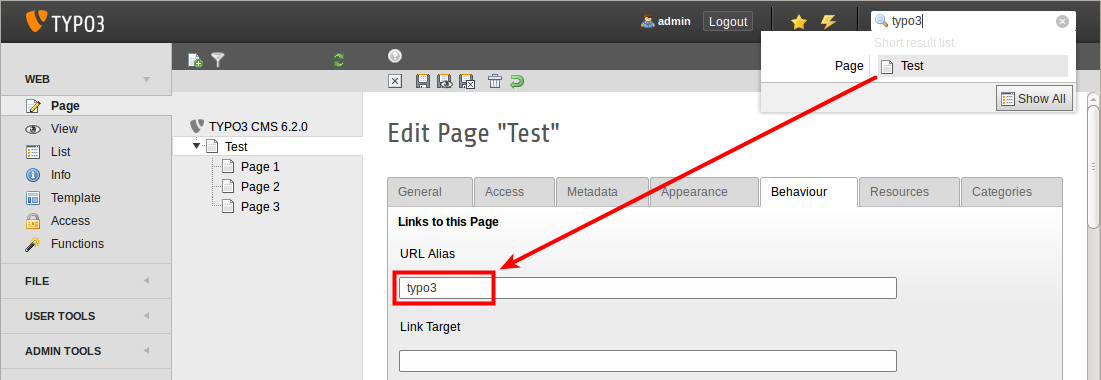
\includegraphics[width=0.95\linewidth]{Images/BackendChanges/LiveSearchInAlias.png}
	\end{figure}

\end{frame}

% ------------------------------------------------------------------------------
% File Abstraction Layer
% ------------------------------------------------------------------------------

\begin{frame}[fragile]
	\frametitle{Изменение во внутреннем интерфейсе}
	\framesubtitle{File Abstraction Layer}

	\begin{itemize}
		\item Название файла и заголовок выводятся в заголовке элемента FAL
	\end{itemize}

	\begin{figure}
		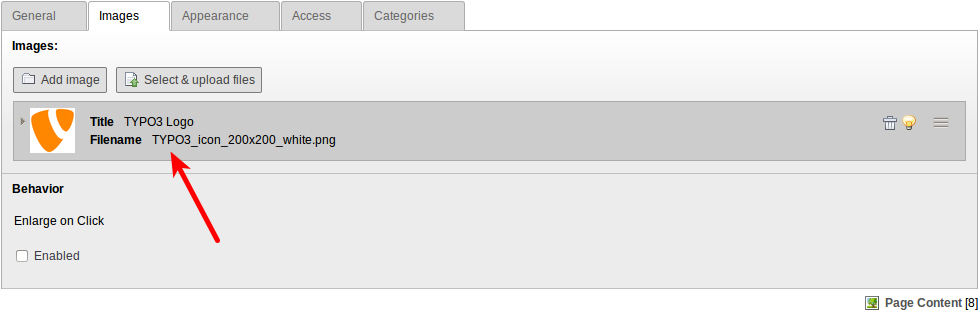
\includegraphics[width=0.95\linewidth]{Images/BackendChanges/FalTitleAndFilename.png}
	\end{figure}

\end{frame}

% ------------------------------------------------------------------------------
% File Abstraction Layer
% ------------------------------------------------------------------------------

\begin{frame}[fragile]
	\frametitle{Изменение во внутреннем интерфейсе}
	\framesubtitle{File Abstraction Layer (EXT:filemetadata)}

	\begin{itemize}
		\item EXT:filemetadata добавляет вкладки для вывода meta информации\newline
			\small(по умолчанию расширение не установлено)\normalsize
	\end{itemize}

	\begin{figure}
		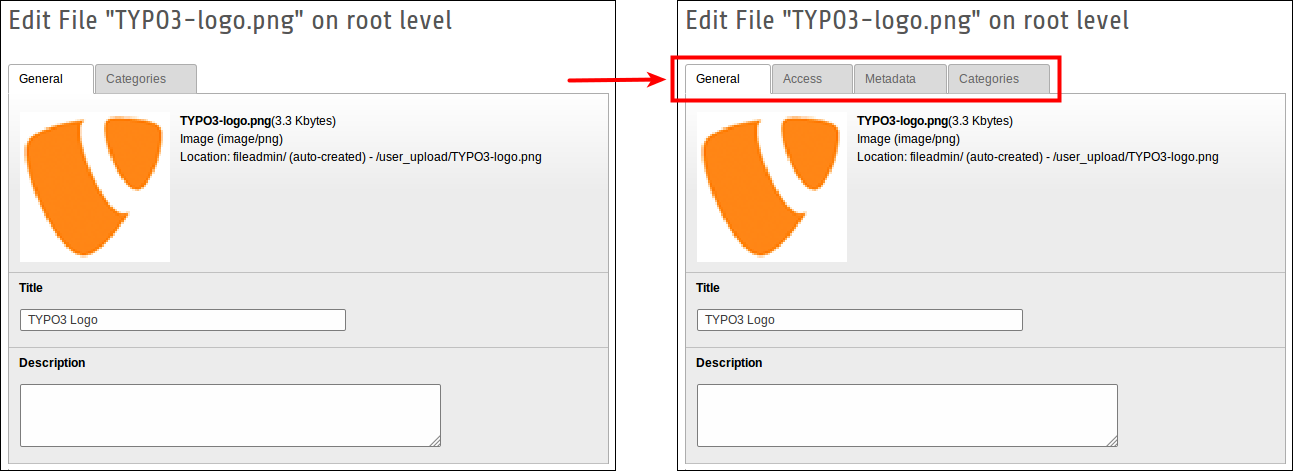
\includegraphics[width=0.95\linewidth]{Images/BackendChanges/FileMetaDataTabs.png}
	\end{figure}

\end{frame}

% ------------------------------------------------------------------------------
% File Abstraction Layer
% ------------------------------------------------------------------------------

\begin{frame}[fragile]
	\frametitle{Изменение во внутреннем интерфейсе}
	\framesubtitle{File Abstraction Layer (EXT:filemetadata)}

	\begin{figure}
		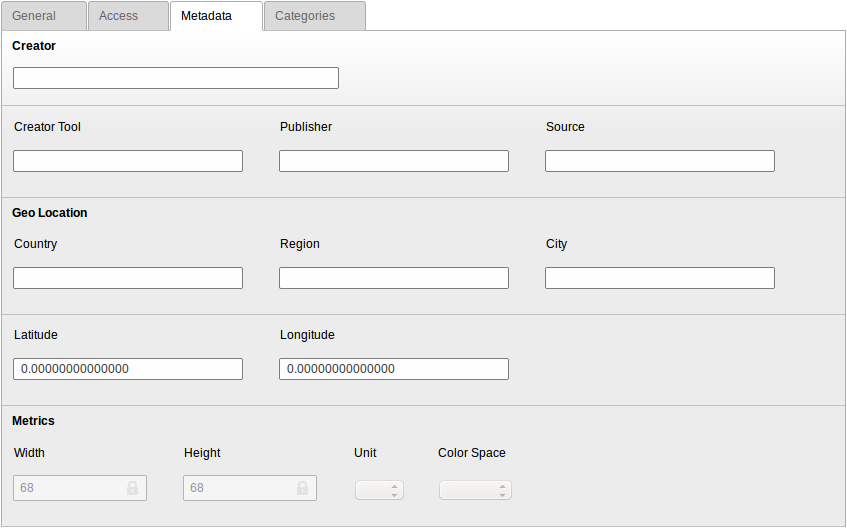
\includegraphics[width=0.8\linewidth]{Images/BackendChanges/FileMetaData.png}
	\end{figure}

\end{frame}


% ------------------------------------------------------------------------------
% File Abstraction Layer
% ------------------------------------------------------------------------------

\begin{frame}[fragile]
	\frametitle{Изменение во внутреннем интерфейсе}
	\framesubtitle{File Abstraction Layer}

	\begin{itemize}
		\item Теперь возможен перевод FAL meta данных на используемые на сайте языки
	\end{itemize}

	\begin{figure}
		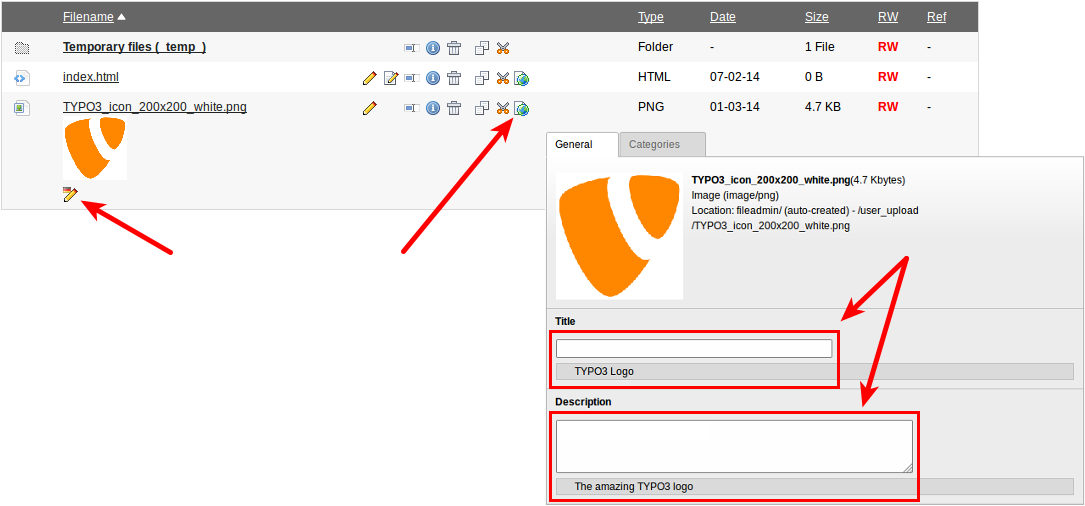
\includegraphics[width=0.95\linewidth]{Images/BackendChanges/FalTranslateMetaData.png}
	\end{figure}

\end{frame}

% ------------------------------------------------------------------------------
% Module: Documentation
% ------------------------------------------------------------------------------

\begin{frame}[fragile]
	\frametitle{Изменение во внутреннем интерфейсе}
	\framesubtitle{Модуль: документация (documentation)}

	\begin{columns}[T]

		\begin{column}{.5\textwidth}
			\begin{itemize}
				\item Модуль "Документация"/"Documentation" позволяет внутренним пользователям загружать и просматривать
				руководства
				\item По умолчанию модуль уже загружен в новых инсталяциях TYPO3
				\item В обновлённых инсталяциях TYPO3 для установки "Документация"/"Documentation" используйте модуль
				управления расширениями
				\item Функция "Управление документацией"/"Manage Documentation" загружает руководства (см. рисунок)
			\end{itemize}
		\end{column}

		\begin{column}{.5\textwidth}
			\begin{figure}\vspace*{-0.4cm}
				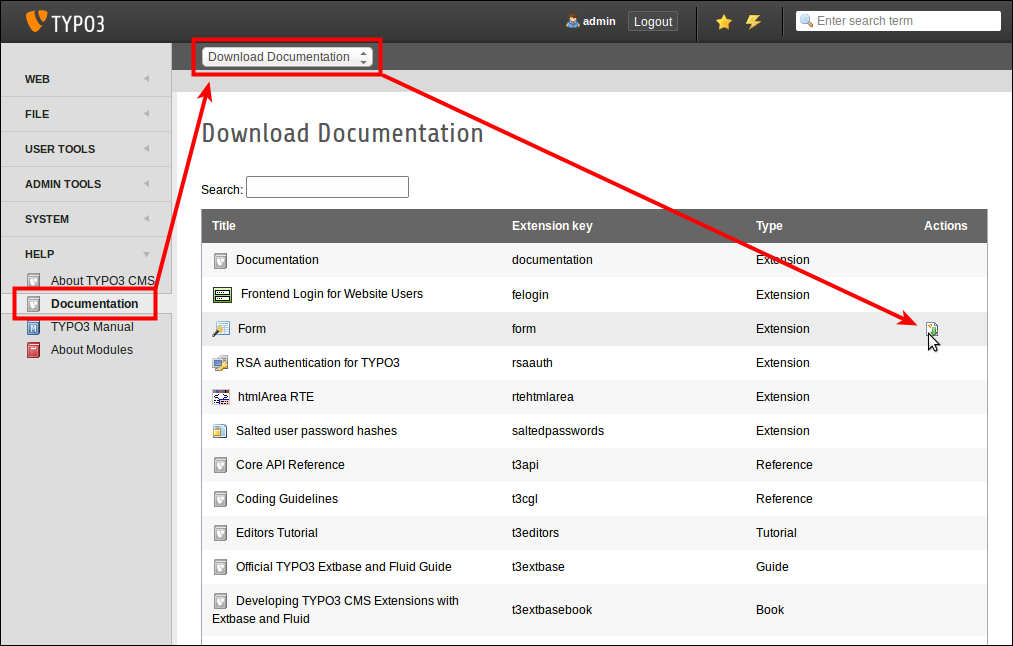
\includegraphics[width=1\linewidth]{Images/BackendChanges/DownloadDocumentation.png}
			\end{figure}
		\end{column}

	\end{columns}

\end{frame}

% ------------------------------------------------------------------------------
% Module: Documentation
% ------------------------------------------------------------------------------

\begin{frame}[fragile]
	\frametitle{Изменение во внутреннем интерфейсе}
	\framesubtitle{Модуль: документация (documentation)}

	\begin{itemize}
		\item Функция "Показать документацию"/"Show Documentation" выводит загруженные документы
	\end{itemize}

	\begin{figure}
		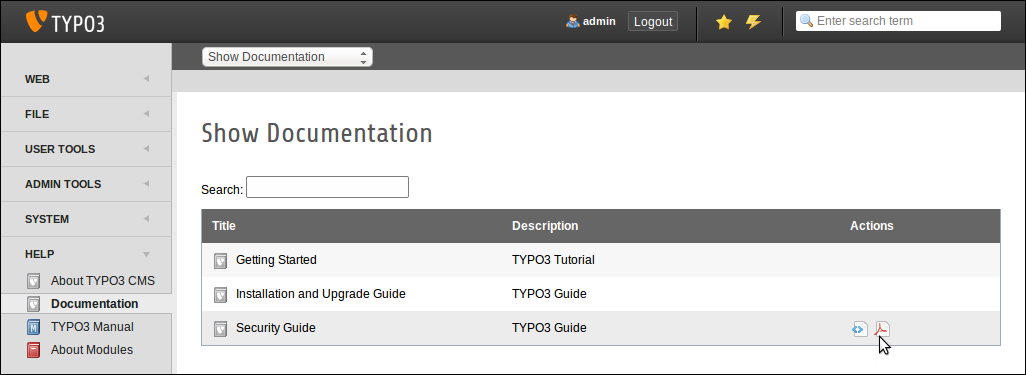
\includegraphics[width=0.95\linewidth]{Images/BackendChanges/ShowDocumentation.png}
	\end{figure}

\end{frame}

% ------------------------------------------------------------------------------
% Removed: TypoScript Help
% ------------------------------------------------------------------------------
% http://forge.typo3.org/issues/47931

\begin{frame}[fragile]
	\frametitle{Изменение во внутреннем интерфейсе}
	\framesubtitle{Удалено: Справка TypoScript/TypoScript Help}

 	\begin{itemize}
		\item EXT:tsconfig\_help ("TSconfig Quick Reference") удален\newline
			\small(устаревшая информация, не обновляемая со времен TYPO3 CMS 4.1)
	\end{itemize}

	\begin{figure}
		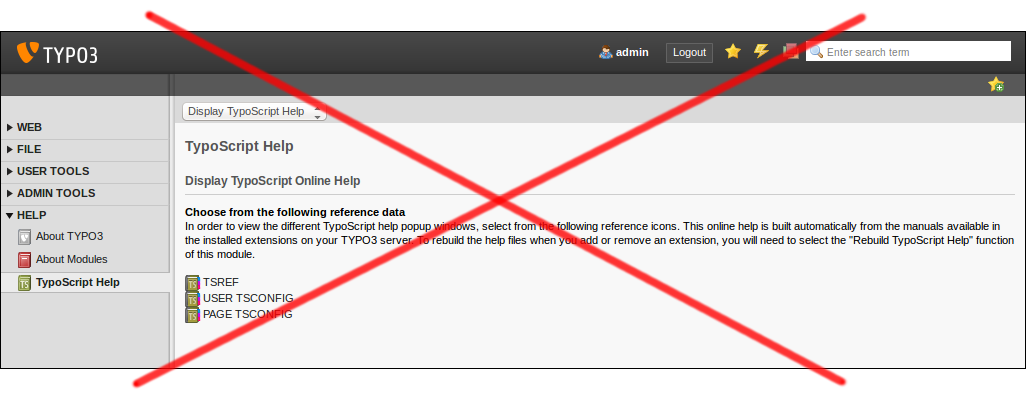
\includegraphics[width=0.95\linewidth]{Images/BackendChanges/TypoScriptHelpRemovedCrossed.png}
	\end{figure}

\end{frame}


% ------------------------------------------------------------------------------
% Scheduler
% ------------------------------------------------------------------------------

\begin{frame}[fragile]
	\frametitle{Изменение во внутреннем интерфейсе}
	\framesubtitle{Планировщик/Scheduler}

	\begin{itemize}
		\item Удаление запланированных задач в режиме правки\newline
			\small(в TYPO3 < 6.2, функция удаления была доступна лишь в режиме списка)\normalsize
	\end{itemize}

	\begin{figure}
		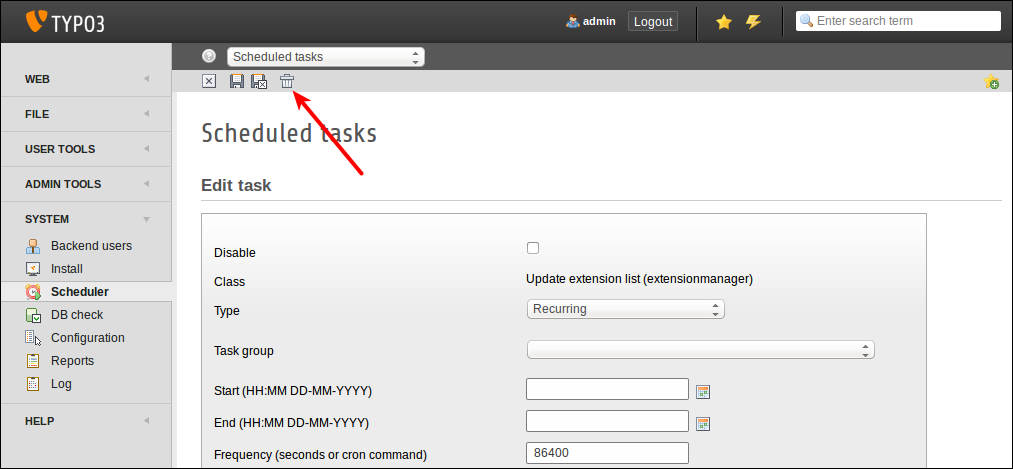
\includegraphics[width=0.95\linewidth]{Images/BackendChanges/DeleteSchedulerTaskInEditView.png}
	\end{figure}

\end{frame}

% ------------------------------------------------------------------------------
% Scheduler
% ------------------------------------------------------------------------------

\begin{frame}[fragile]
	\frametitle{Изменение во внутреннем интерфейсе}
	\framesubtitle{Планировщик/Scheduler}

	\begin{itemize}
		\item К запланированной задаче можно прикрепить описание, которое выводится в виде подзаголовка в режиме списка,
		либо как подсказка (на следующем слайде)
	\end{itemize}

	\begin{figure}
		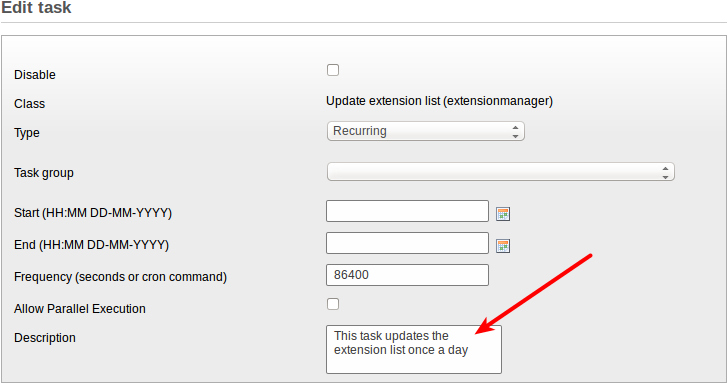
\includegraphics[width=0.7\linewidth]{Images/BackendChanges/SchedulerTaskDescription.png}
	\end{figure}

\end{frame}

% ------------------------------------------------------------------------------
% Scheduler
% ------------------------------------------------------------------------------

\begin{frame}[fragile]
	\frametitle{Изменение во внутреннем интерфейсе}
	\framesubtitle{Планировщик/Scheduler}

	\begin{itemize}
		\item Описание задачи в виде подзаголовка\newline
			\small(необходимо включение в настройке расширения)\normalsize
	\end{itemize}

	\begin{figure}
		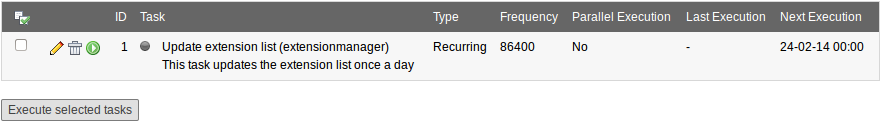
\includegraphics[width=0.95\linewidth]{Images/BackendChanges/SchedulerTaskDescriptionAsSubheader.png}
	\end{figure}


	\begin{itemize}
		\item Описание задачи в виде подсказки ("hover")
	\end{itemize}

	\begin{figure}
		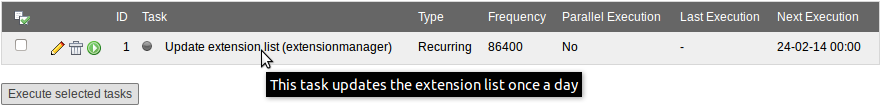
\includegraphics[width=0.95\linewidth]{Images/BackendChanges/SchedulerTaskDescriptionAsTooltip.png}
	\end{figure}

\end{frame}

% ------------------------------------------------------------------------------
% Scheduler
% ------------------------------------------------------------------------------

\begin{frame}[fragile]
	\frametitle{Изменение во внутреннем интерфейсе}
	\framesubtitle{Планировщик/Scheduler}

	\begin{itemize}
		\item Теперь возможна группировка планируемых задач
		\item Добавляйте записи "группа плановых задач"/"scheduler task group" на корневую страницу (UID: 0) и выбирайте группу
		 в задаче
	\end{itemize}

	\begin{figure}
		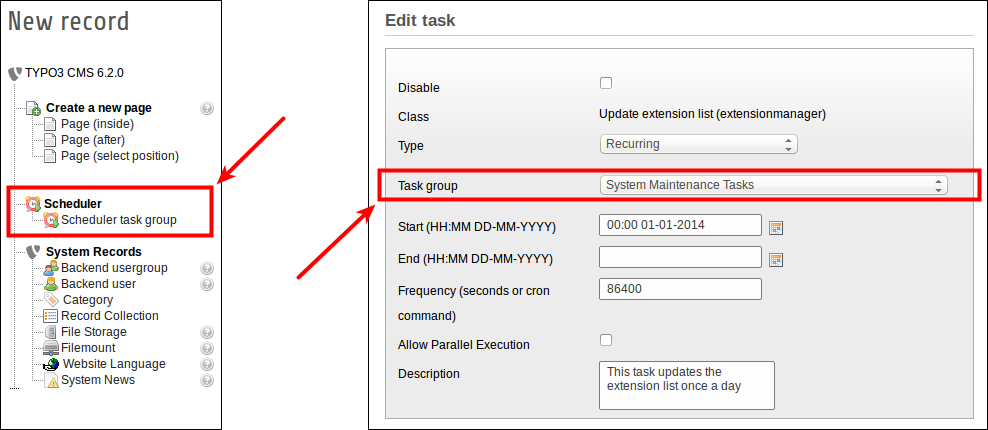
\includegraphics[width=0.85\linewidth]{Images/BackendChanges/SchedulerTaskGroup.png}
	\end{figure}

\end{frame}

% ------------------------------------------------------------------------------
% System Extension: Form
% ------------------------------------------------------------------------------
% http://forge.typo3.org/issues/38094

\begin{frame}[fragile]
	\frametitle{Изменение во внутреннем интерфейсе}
	\framesubtitle{Системное расширение: Формы/Form}

		\begin{columns}[T]

    		\begin{column}{.5\textwidth}
				\begin{itemize}
					\item Новая пост обработка для cObject FORM: \textbf{redirect}\newline
						(перенаправление после подтверждения формы)
					\item Значение анализируется в \texttt{typolink} (функция TypoScript),\newline
						то есть значение может быть и ID страницы, и URL
				\end{itemize}
    		\end{column}

    		\begin{column}{.5\textwidth}
    			\begin{figure}\vspace*{-0.4cm}
    				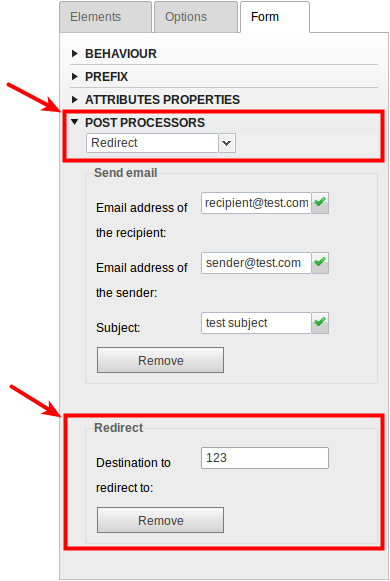
\includegraphics[width=0.65\linewidth]{Images/BackendChanges/FormRedirectPostProcessor.png}
    			\end{figure}
    		\end{column}

    	\end{columns}

\end{frame}

% ------------------------------------------------------------------------------
% Module: List
% ------------------------------------------------------------------------------
% http://forge.typo3.org/issues/49810

\begin{frame}[fragile]
	\frametitle{Изменение во внутреннем интерфейсе}
	\framesubtitle{Модуль Список/List}

	\begin{itemize}
		\item Дополнительные столбцы "UID" и "PID" в режиме списка для не администраторов/admins
	\end{itemize}

	\begin{figure}
		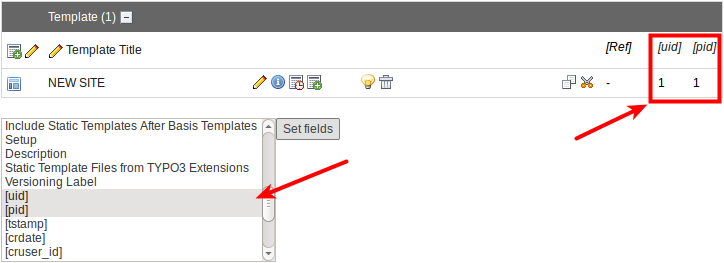
\includegraphics[width=0.95\linewidth]{Images/BackendChanges/AdditionalColumnsInListModule.png}
	\end{figure}

\end{frame}

% ------------------------------------------------------------------------------
% File Abstraction Layer
% ------------------------------------------------------------------------------
% http://forge.typo3.org/issues/50827
% http://forge.typo3.org/issues/51097

\begin{frame}[fragile]
	\frametitle{Изменение во внутреннем интерфейсе}
	\framesubtitle{File Abstraction Layer}

	\begin{itemize}
		\item Если при индексации обнаружен файл с ошибкой, выводится сообщение и устанавливается флаг для записи в БД
		\item Это отображается и в модуле "Отчеты"/"Reports"
		\item Если же файл снова появляется, сообщение и флаг сбрасываются
	\end{itemize}

	\begin{columns}[T]

		\begin{column}{.5\textwidth}
			\begin{figure}
				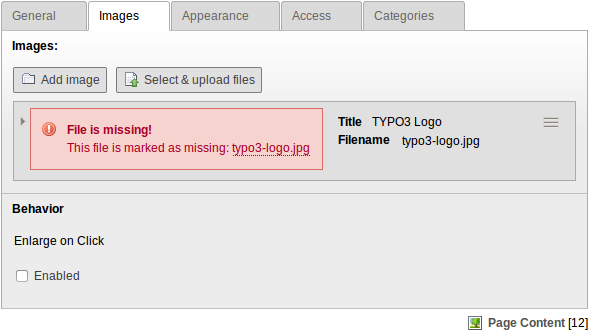
\includegraphics[width=0.95\linewidth]{Images/BackendChanges/FalMissingFileContentElement.png}
			\end{figure}
		\end{column}

		\begin{column}{.5\textwidth}
			\begin{figure}
				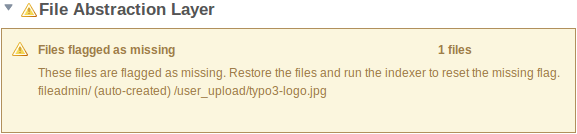
\includegraphics[width=0.95\linewidth]{Images/BackendChanges/FalMissingFileReportsModule.png}
			\end{figure}
		\end{column}

	\end{columns}

\end{frame}

% ------------------------------------------------------------------------------
% Menu/Sitemap: Categories-based Menus
% ------------------------------------------------------------------------------
% http://forge.typo3.org/issues/51161

\begin{frame}[fragile]
	\frametitle{Изменение во внутреннем интерфейсе}
	\framesubtitle{Меню категорий (1)}

	\begin{itemize}
		\item Элемент содержимого "Меню/Карта сайта"/"Menu/Sitemap" теперь может создавать меню категорий
	\end{itemize}

	\begin{figure}
		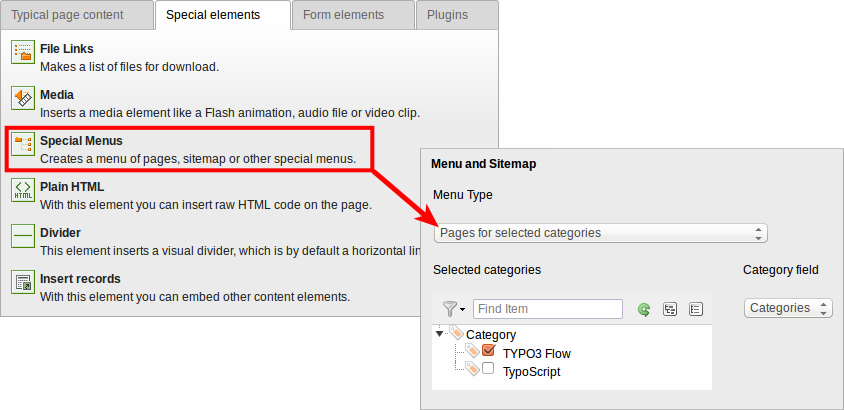
\includegraphics[width=0.8\linewidth]{Images/BackendChanges/CategoryBasedMenus.png}
	\end{figure}

\end{frame}

% ------------------------------------------------------------------------------
% Menu/Sitemap: Category-based Menus
% (slide added in March 2014)
% ------------------------------------------------------------------------------


\begin{frame}[fragile]
	\frametitle{Изменение во внутреннем интерфейсе}
	\framesubtitle{Меню категорий (2)}

	\begin{itemize}
		\item Другой тип нового меню: "\underline{Элементы содержимого} из выбранных категорий"
	\end{itemize}

	\begin{figure}
		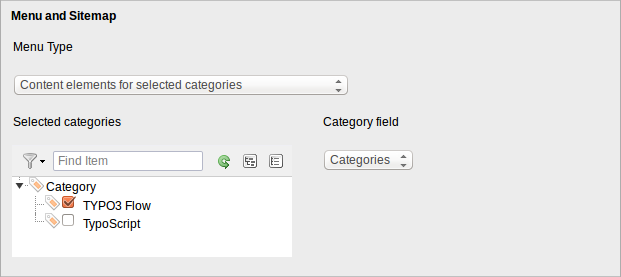
\includegraphics[width=0.6\linewidth]{Images/BackendChanges/ContentElementsForSelectedCategories.png}
	\end{figure}

\end{frame}

% ------------------------------------------------------------------------------
% Sorting Categories
% ------------------------------------------------------------------------------
% http://forge.typo3.org/issues/51590

\begin{frame}[fragile]
	\frametitle{Изменение во внутреннем интерфейсе}
	\framesubtitle{Упорядочивание категорий}

 	\begin{itemize}
		\item Теперь категории можно упорядочить\newline
			\small(в TYPO3 < 6.2, категории всегда выводились по алфавиту)\normalsize
	\end{itemize}

	\begin{figure}
		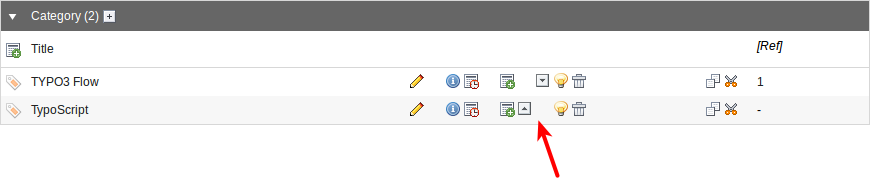
\includegraphics[width=0.95\linewidth]{Images/BackendChanges/CategorySorting.png}
	\end{figure}

\end{frame}

% ------------------------------------------------------------------------------
% Category Visibility
% ------------------------------------------------------------------------------
% http://forge.typo3.org/issues/52718

\begin{frame}[fragile]
	\frametitle{Изменение во внутреннем интерфейсе}
	\framesubtitle{Видимость категорий}

 	\begin{itemize}
		\item Для внутренних пользователей/групп можно ограничить видимость категорий
		users/groups
	\end{itemize}

	\begin{figure}
		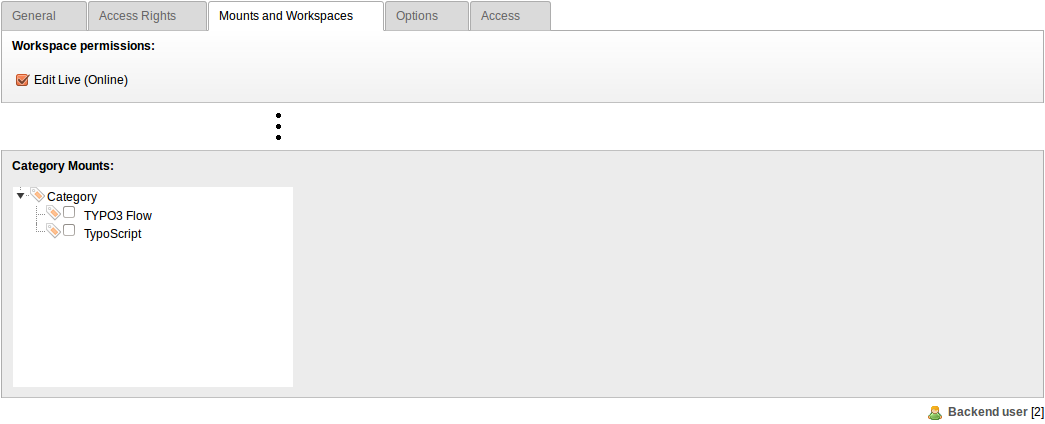
\includegraphics[width=0.95\linewidth]{Images/BackendChanges/CategoryVisibility.png}
	\end{figure}

\end{frame}

% ------------------------------------------------------------------------------
% "New Content" icon always visible
% ------------------------------------------------------------------------------
% http://forge.typo3.org/issues/48938
% http://forge.typo3.org/issues/51480

\begin{frame}[fragile]
	\frametitle{Изменение во внутреннем интерфейсе}
	\framesubtitle{Удобство}

 	\begin{itemize}
		\item Если столбец пуст, всегда выводиться значок "добавить содержимое"/"new content"\newline
			\small(это помогает редакторам понять, что они могут сделать)\normalsize
	\end{itemize}

	\begin{figure}
		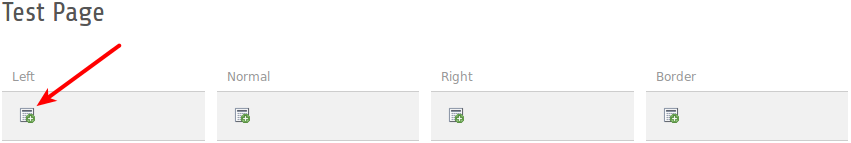
\includegraphics[width=0.95\linewidth]{Images/BackendChanges/NewContentIconAlwaysVisible.png}
	\end{figure}

\end{frame}

% ------------------------------------------------------------------------------
% Module "Functions": Hide In Menus
% ------------------------------------------------------------------------------
% http://forge.typo3.org/issues/51017

\begin{frame}[fragile]
	\frametitle{Изменение во внутреннем интерфейсе}
	\framesubtitle{Функции}

    \begin{itemize}
		\item При создании нескольких страниц в модуле "функции"/"functions", новый флажок позволяет редакторам скрыть
		эти страницы в меню
		\smallОчень полезно при создании множества страниц за раз\normalsize
	\end{itemize}

	\begin{figure}
		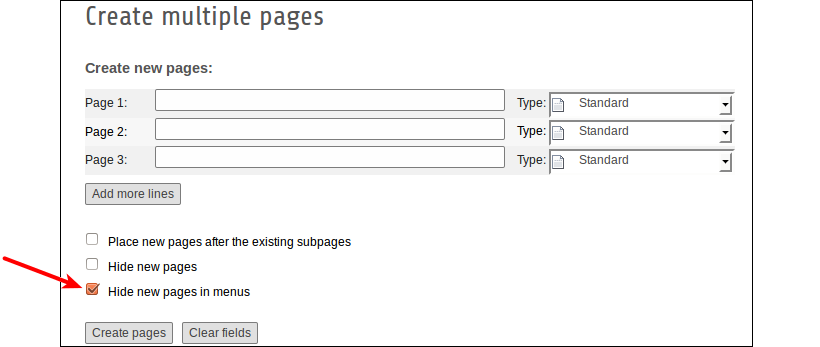
\includegraphics[width=0.85\linewidth]{Images/BackendChanges/CreateMultiplePagesHideInMenu.png}
	\end{figure}

\end{frame}

% ------------------------------------------------------------------------------
% Extension Manager: Upload Extensions
% ------------------------------------------------------------------------------
% http://forge.typo3.org/issues/51776
% http://forge.typo3.org/issues/51437

\begin{frame}[fragile]
	\frametitle{Изменение во внутреннем интерфейсе}
	\framesubtitle{Управление расширениями}

 	\begin{itemize}
		\item Загрузка расширений посредством функции "Получить расширение"/"Get Extensions"
	\end{itemize}

	\begin{figure}
		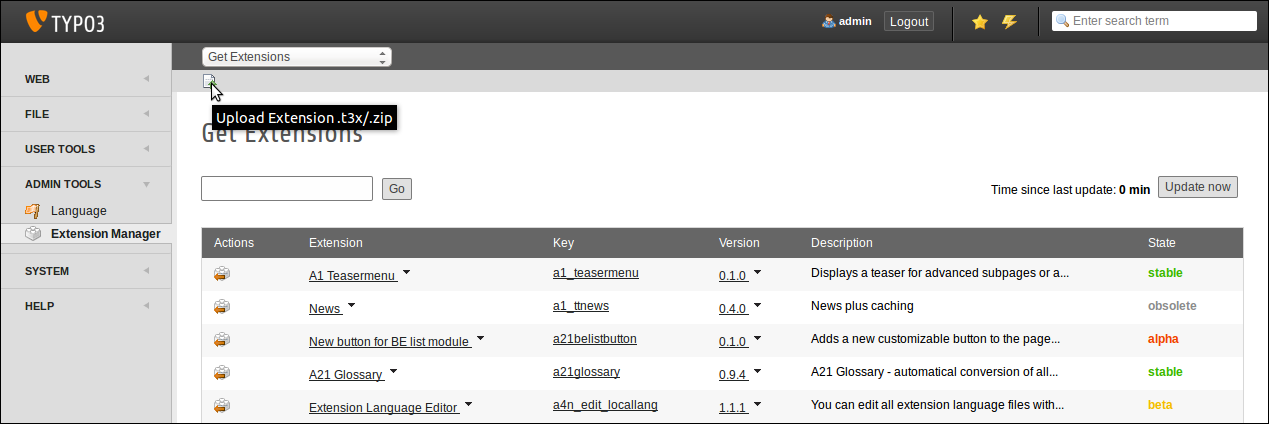
\includegraphics[width=0.95\linewidth]{Images/BackendChanges/UploadExtension.png}
	\end{figure}

\end{frame}

% ------------------------------------------------------------------------------
% Recycler
% ------------------------------------------------------------------------------
% http://forge.typo3.org/issues/52324

\begin{frame}[fragile]
	\frametitle{Изменение во внутреннем интерфейсе}
	\framesubtitle{Корзина}

 	\begin{itemize}
		\item Записи в корзине можно упорядочить по времени\newline
			\small(что помогает пользователям решить, какую запись нужно восстановить)\normalsize
	\end{itemize}

	\begin{figure}
		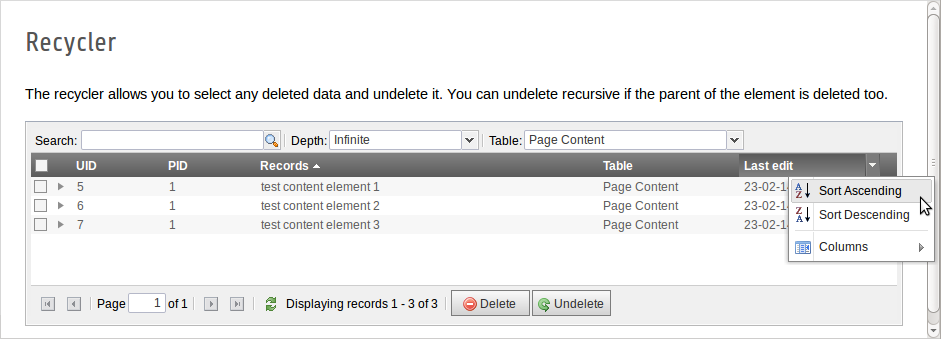
\includegraphics[width=0.95\linewidth]{Images/BackendChanges/RecyclerSortRecord.png}
	\end{figure}

\end{frame}

% ------------------------------------------------------------------------------
% File/Directory Permissions
% ------------------------------------------------------------------------------

\begin{frame}[fragile]
	\frametitle{Изменение во внутреннем интерфейсе}
	\framesubtitle{Разрешения для Файлов/Директорий}

    \begin{itemize}
		\item Гораздо более детальная настройка разрешений для файлов/директория для внутренних пользователей/групп
			\begingroup\color{typo3red}\textbf{(1)}\endgroup
		\item Возможно, начиная с TYPO3 6.0, но только через UserTSconfig
			\begingroup\color{typo3red}\textbf{(2)}\endgroup
	\end{itemize}

	\begin{figure}
		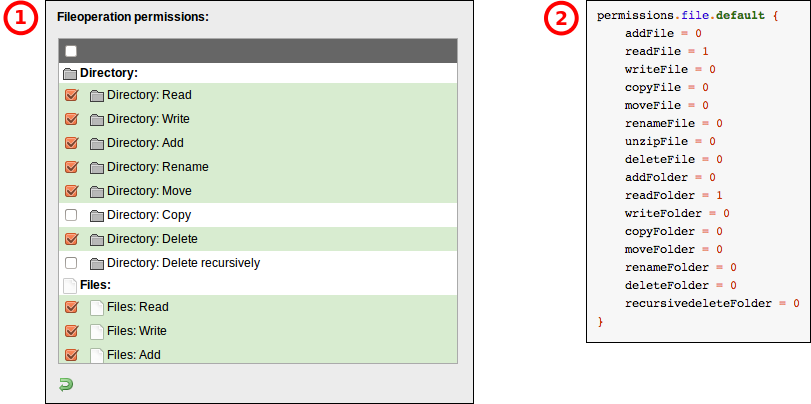
\includegraphics[width=0.75\linewidth]{Images/BackendChanges/FileAndDirectoryPermissions.png}
	\end{figure}

\end{frame}

% ------------------------------------------------------------------------------
% OpenID
% ------------------------------------------------------------------------------

\begin{frame}[fragile]
	\frametitle{Изменение во внутреннем интерфейсе}
	\framesubtitle{OpenID (1)}

 	\begin{itemize}
		\item OpenID для авторизации внутренних пользователей можно настроить через мастер
		\item Для этого потребуется установить EXT:openid (системное расширение)
	\end{itemize}

	\begin{figure}
		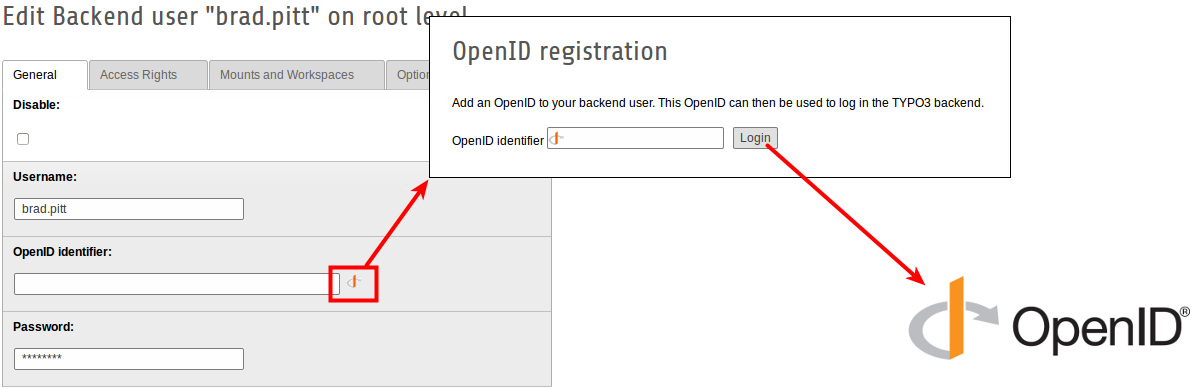
\includegraphics[width=0.95\linewidth]{Images/BackendChanges/OpenIdWizard.png}
	\end{figure}

\end{frame}

% ------------------------------------------------------------------------------
% OpenID
% ------------------------------------------------------------------------------

\begin{frame}[fragile]
	\frametitle{Изменение во внутреннем интерфейсе}
	\framesubtitle{OpenID (2)}

 	\begin{itemize}
		\item OpenID для авторизации внутренних пользователей можно настроить через мастер
		\item Для этого потребуется установить EXT:openid (системное расширение)
	\end{itemize}

	\begin{figure}
		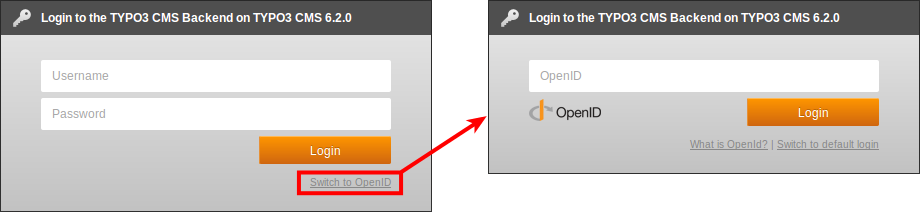
\includegraphics[width=0.8\linewidth]{Images/BackendChanges/OpenIdLogin.png}
	\end{figure}

 	\begin{itemize}
		\item Дополнительно об OpenID:\newline
			\small\url{http://openid.net}\normalsize
	\end{itemize}


\end{frame}

% ------------------------------------------------------------------------------
% Workspaces
% ------------------------------------------------------------------------------
% http://forge.typo3.org/issues/50223
% http://forge.typo3.org/issues/50224

\begin{frame}[fragile]
	\frametitle{Изменение во внутреннем интерфейсе}
	\framesubtitle{Рабочие области/Workspaces}

 	\begin{itemize}
		\item Редакторы/пользователи могут определять кого извещать, без ограничения со стороны системы
		\item Вкладка "Все"/"All" теперь видна для \underline{всех} пользователей
	\end{itemize}

	\begin{figure}
		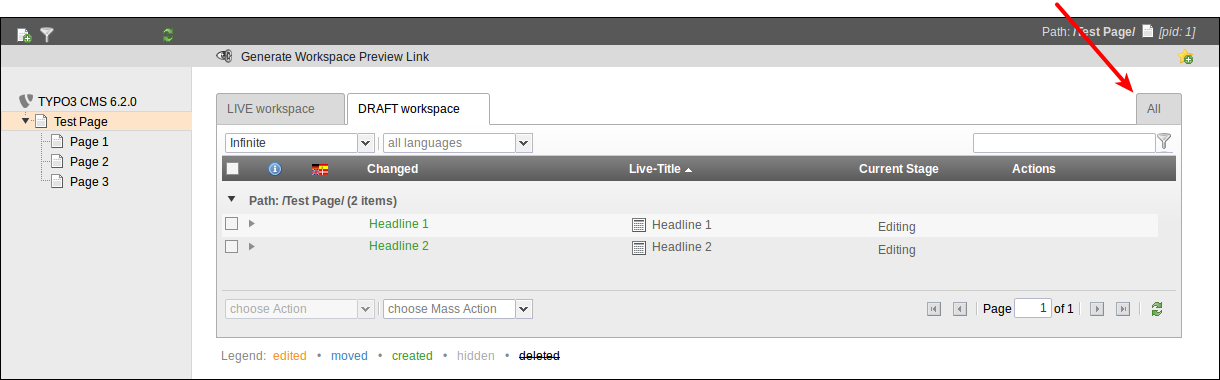
\includegraphics[width=0.95\linewidth]{Images/BackendChanges/WorkspacesTabAll.png}
	\end{figure}

\end{frame}

% ------------------------------------------------------------------------------

